\chapter{Experimentos e resultados}
\label{chap:Experimentos e resultados}
\lettrine{N}{este} capítulo presentaranse os experimentos realizados e os resultados obtidos.
Para iso, comezarase presentando unha vista xeral do proceso de experimentación, 
A continuación, presentaranse os resultados obtidos cas diferentes configuracións probadas.

\section{Vista Xeral}
\label{sec:Vista Xeral}

Diferentes funciones de loss 
    - ncc, ssmi

\section{Estratexias de mostraxe}
\label{sec:Estratexias de mostraxe}

Orixinalmente IDIR utiliza unha estratexia de mostraxe aleatoria para seleccionar os puntos que se pasan á rede en cada iteración.
Mentres que esta estretexia parece suficiente para o rexitro de pulmóns, no caso das imaxes de retina isto non ten porque ser así.
Isto debe a que as imaxes de retina teñen seccións con moita mais información que outras, frente os CTs de pulmóns que está moita mais repartida.
Ademais, teñen maiores desprazamentos e menor superposición entre cada parella. 

Para solucionar isto, propúxose unha estratexia de mostraxe mais intellixente, onde se calcula unha máscara de probabilidade para cada imaxe, que se utiliza para seleccionar os puntos que se pasan á rede.
Para calcular esta máscara, extráense mediante operadores de Sobel os vasos sanguíneos e mediante umbralización o disco óptico, que son as zonas onde se espera que haxa máis información, e dáselles mais probabilidades de ser seleccionadas.
Esta aproximación estaba errada, \dots

Posteriormente probouse unha estratexia de mostraxe uniforme, onde se seleccionan un número fixo de puntos en cada imaxe, independentemente da información que conteña.
É unha estratexia similar ao mostraxe aleatorio, pero garantindo que se cubre a maior parte posible da imaxe. Isto é importante en experimentos con batch sizes pequenos.
A implementación non foi moi sinxela xa que repartir uniformemente un número arbitrario de puntos dentro duncha máscara circular (mais non perfectamente circular) non é tan trivial como repartilos nunha máscara rectangular.

Así mesmo implementouse un scheduling do batch size, coa intención de utilizar poucos puntos inicialmente para que a rede aprenda a transformación global, e aumentar o número de puntos conforme avanzase o entrenamento para que a rede aprenda as transformación locais.

\begin{figure}[]
    \centering
    \begin{subfigure}[b]{0.3\textwidth}
        \centering
        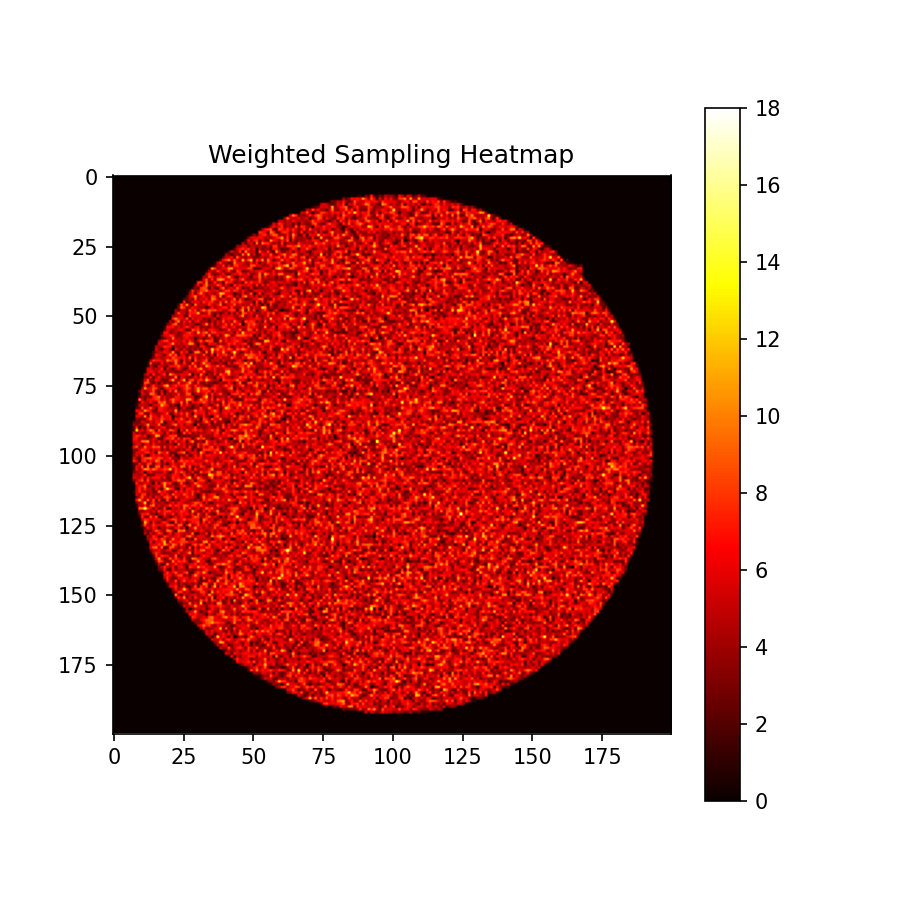
\includegraphics[width=\textwidth]{imaxes/random_sampling_heatmap.png}
        \caption{Heatmap de mostraxe aleatorio}
        \label{fig:random_sampling_heatmap}
    \end{subfigure}
    \hfill
    \begin{subfigure}[b]{0.3\textwidth}
        \centering
        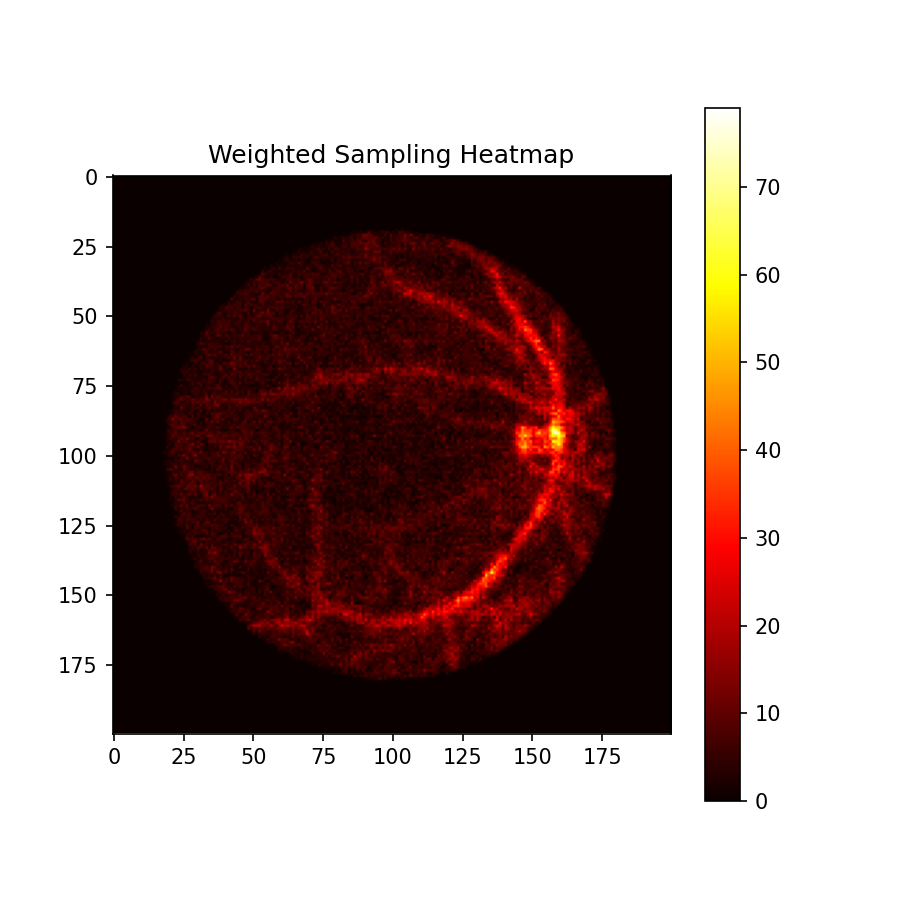
\includegraphics[width=\textwidth]{imaxes/weighted_sampling_heatmap.png}
        \caption{Heatmap de mostraxe con peso}
        \label{fig:weighted_sampling_heatmap}
    \end{subfigure}
    \hfill
    \begin{subfigure}[b]{0.3\textwidth}
        \centering
        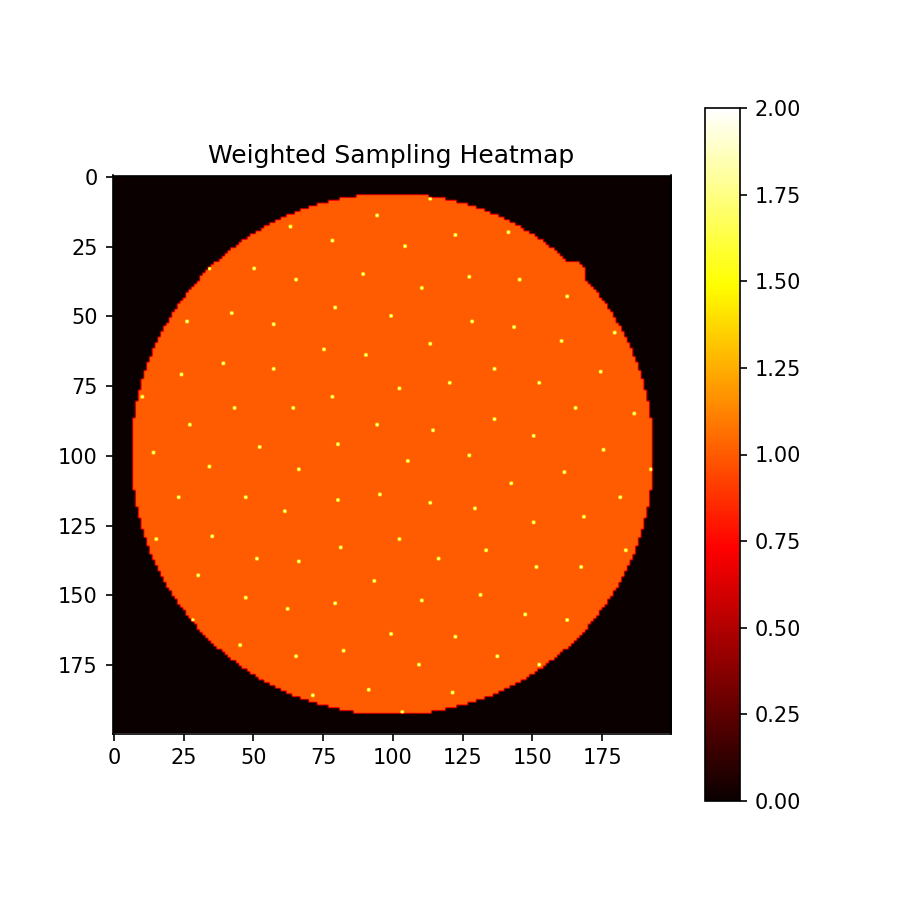
\includegraphics[width=\textwidth]{imaxes/uniform_sampling_heatmap.png}
        \caption{Heatmap de mostraxe uniforme (100 puntos)}
        \label{fig:uniform_sampling_heatmap}
    \end{subfigure}
    \caption{Heatmaps de mostraxe}
    \label{fig:sampling_heatmaps}
\end{figure}

